\documentclass[]{book}
\usepackage{lmodern}
\usepackage{amssymb,amsmath}
\usepackage{ifxetex,ifluatex}
\usepackage{fixltx2e} % provides \textsubscript
\ifnum 0\ifxetex 1\fi\ifluatex 1\fi=0 % if pdftex
  \usepackage[T1]{fontenc}
  \usepackage[utf8]{inputenc}
\else % if luatex or xelatex
  \ifxetex
    \usepackage{mathspec}
  \else
    \usepackage{fontspec}
  \fi
  \defaultfontfeatures{Ligatures=TeX,Scale=MatchLowercase}
\fi
% use upquote if available, for straight quotes in verbatim environments
\IfFileExists{upquote.sty}{\usepackage{upquote}}{}
% use microtype if available
\IfFileExists{microtype.sty}{%
\usepackage{microtype}
\UseMicrotypeSet[protrusion]{basicmath} % disable protrusion for tt fonts
}{}
\usepackage[margin=1in]{geometry}
\usepackage{hyperref}
\hypersetup{unicode=true,
            pdftitle={Applied Time Series Analysis},
            pdfauthor={Vipul Bhatt},
            pdfborder={0 0 0},
            breaklinks=true}
\urlstyle{same}  % don't use monospace font for urls
\usepackage{natbib}
\bibliographystyle{apalike}
\usepackage{longtable,booktabs}
\usepackage{graphicx,grffile}
\makeatletter
\def\maxwidth{\ifdim\Gin@nat@width>\linewidth\linewidth\else\Gin@nat@width\fi}
\def\maxheight{\ifdim\Gin@nat@height>\textheight\textheight\else\Gin@nat@height\fi}
\makeatother
% Scale images if necessary, so that they will not overflow the page
% margins by default, and it is still possible to overwrite the defaults
% using explicit options in \includegraphics[width, height, ...]{}
\setkeys{Gin}{width=\maxwidth,height=\maxheight,keepaspectratio}
\IfFileExists{parskip.sty}{%
\usepackage{parskip}
}{% else
\setlength{\parindent}{0pt}
\setlength{\parskip}{6pt plus 2pt minus 1pt}
}
\setlength{\emergencystretch}{3em}  % prevent overfull lines
\providecommand{\tightlist}{%
  \setlength{\itemsep}{0pt}\setlength{\parskip}{0pt}}
\setcounter{secnumdepth}{5}
% Redefines (sub)paragraphs to behave more like sections
\ifx\paragraph\undefined\else
\let\oldparagraph\paragraph
\renewcommand{\paragraph}[1]{\oldparagraph{#1}\mbox{}}
\fi
\ifx\subparagraph\undefined\else
\let\oldsubparagraph\subparagraph
\renewcommand{\subparagraph}[1]{\oldsubparagraph{#1}\mbox{}}
\fi

%%% Use protect on footnotes to avoid problems with footnotes in titles
\let\rmarkdownfootnote\footnote%
\def\footnote{\protect\rmarkdownfootnote}

%%% Change title format to be more compact
\usepackage{titling}

% Create subtitle command for use in maketitle
\newcommand{\subtitle}[1]{
  \posttitle{
    \begin{center}\large#1\end{center}
    }
}

\setlength{\droptitle}{-2em}

  \title{Applied Time Series Analysis}
    \pretitle{\vspace{\droptitle}\centering\huge}
  \posttitle{\par}
    \author{Vipul Bhatt}
    \preauthor{\centering\large\emph}
  \postauthor{\par}
      \predate{\centering\large\emph}
  \postdate{\par}
    \date{2018-07-20}

\usepackage{booktabs}
\usepackage{amsthm}
\makeatletter
\def\thm@space@setup{%
  \thm@preskip=8pt plus 2pt minus 4pt
  \thm@postskip=\thm@preskip
}
\makeatother

\usepackage{amsthm}
\newtheorem{theorem}{Theorem}[chapter]
\newtheorem{lemma}{Lemma}[chapter]
\theoremstyle{definition}
\newtheorem{definition}{Definition}[chapter]
\newtheorem{corollary}{Corollary}[chapter]
\newtheorem{proposition}{Proposition}[chapter]
\theoremstyle{definition}
\newtheorem{example}{Example}[chapter]
\theoremstyle{definition}
\newtheorem{exercise}{Exercise}[chapter]
\theoremstyle{remark}
\newtheorem*{remark}{Remark}
\newtheorem*{solution}{Solution}
\begin{document}
\maketitle

{
\setcounter{tocdepth}{1}
\tableofcontents
}
\chapter*{Preface}\label{preface}
\addcontentsline{toc}{chapter}{Preface}

These lecture notes are prepared for an upper level undergraduate course
in time series econometrics. Every fall I teach a course on applied time
series analysis at James Madison University. These notes borrow heavliy
from the teaching material that I have developed over several years of
instruction of this course.

One of my main objective is to develop a primer on time series analysis
that is more accessible to undergraduate students than standard
textbooks available in the market. Most of these textbooks in my opinion
are densely written and assume advanced mathematical skills on the part
of our students. Further, I have also struggled with their topic
selection and organization. Often I end up not following the chapters in
order and modify content (by adding or subtracting) to meet my students
needs. Such changes causes confusion for some students and more
importantly discourages optimal use of the textbook. Hence, this is an
undertaking to develop a primer on time series that is accessible,
follows a more logical sequencing of topics, and covers content that is
most useful for undergraduate students in business and economics.

\emph{Note: These notes have been prepared by me using various sources,
published and unpublished. All errors that remain are mine.}

\chapter{Introduction}\label{intro}

A time series is a specific kind of data where observations of a
variable are recorded over time. For example, the data for the U.S. GDP
for the last 30 years is a time series data.

Such data shows how a variable is changing over time. Depending on the
variable of interest we can have data measured at different frequencies.
Some commonly used frequencies are intra-day, daily, weekly, monthly,
quarterly, semi-annual and annual. Figure \ref{fig:figone} below plots
data for quarterly and monthly frequency.

\begin{figure}

{\centering 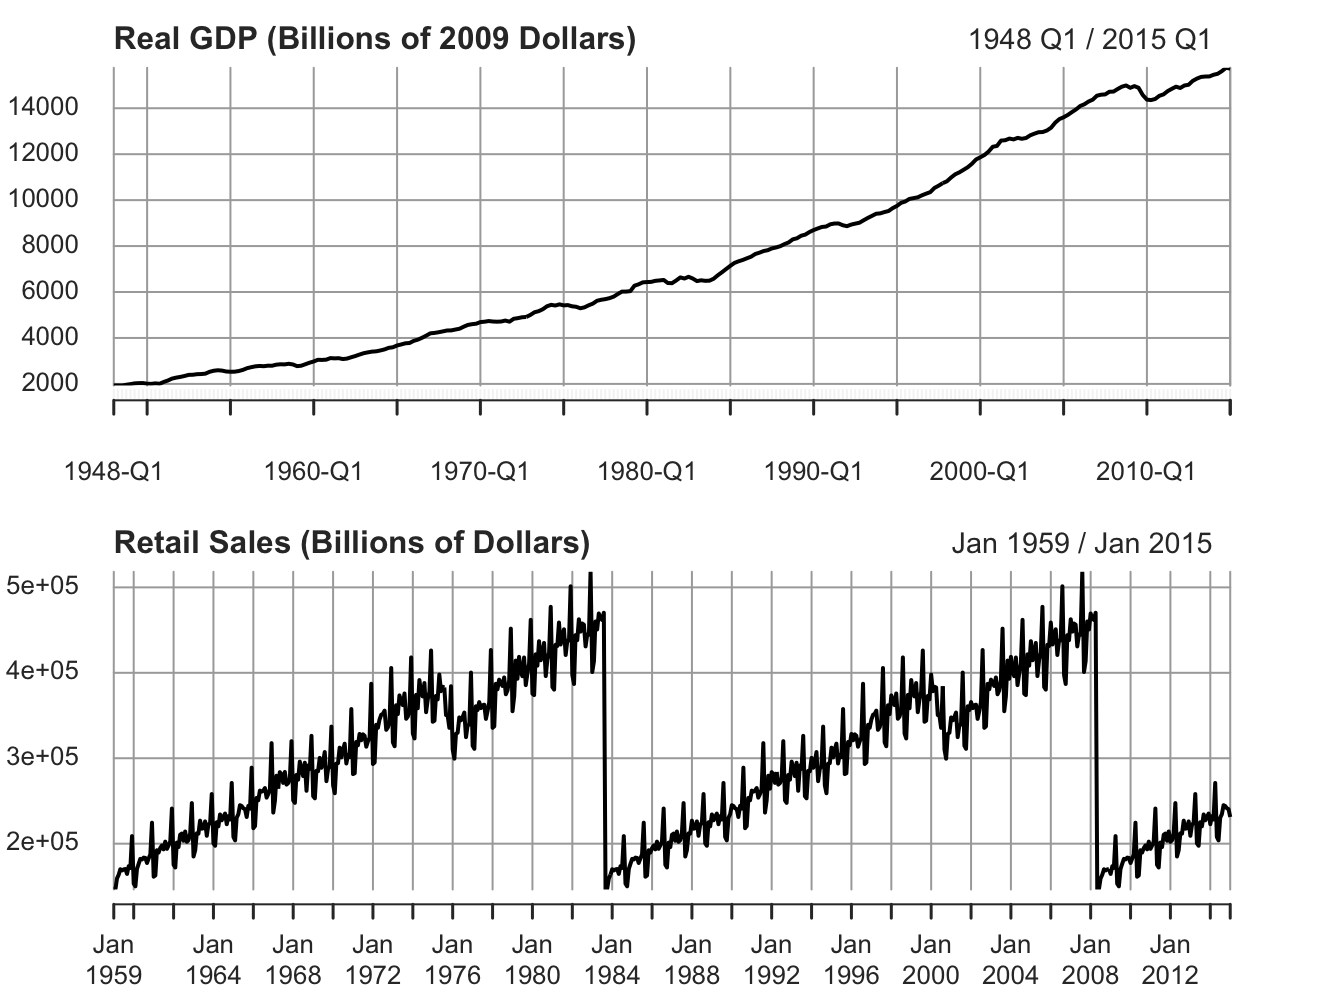
\includegraphics[width=0.8\linewidth]{bookdown-demo_files/figure-latex/figone-1} 

}

\caption{Time Series at quarterly and monthly frequency}\label{fig:figone}
\end{figure}

The first panel shows data for the real gross domestic product (GDP) for
the US in 2009 dollars, measured at a quarterly frequency. The second
panel shows data for the retail sales in the U.S. billions of dollars,
measured at monthly frequency.

Formally, we denote a time series variable by \(x_t\), where
\(t=0,1,2,..,T\) is the observation index. For example, at \(t=10\) we
get the tenth observation of this time series, \(x_{10}\).

\chapter{Smoothing Methods and Regression-based
Forecasting}\label{smoothing-methods-and-regression-based-forecasting}

In this chapter we will look at simple techniques that can be used to
forecast a time series variable. Here we focus on methods that do not
account for various components of a time series explicitly. The list of
tecniques covered in this topic are:

\begin{enumerate}
\def\labelenumi{\arabic{enumi}.}
\tightlist
\item
  Smoothing Methods
\item
  Regressiion-based Forecasting
\end{enumerate}

``Naive Forecasting Methods'' There are many `back-of-envelope' type of
forecasting methods often used by practitioners. For example:

\section{Smoothing Methods}\label{smoothing-methods}

This approach attempts to \emph{average} out the irregular component of
a Time series.

\subsection{Moving Average Method}\label{moving-average-method}

Here we compute an average of most recent data values for the time
series and use it as a forecast for the next period.

An important parameter is the \emph{window} over which we take the
average. Let us denote this window by \(m\), then:

\begin{equation}
    y^f_{T+1}=\frac{\sum_{i=t-m+1}^{t}{y_i}}{m}
    \end{equation}

As we increase \(m\), more weight is given to more recent observations
and hence we get less \emph{smoothing}. A larger value is more desirable
when there are large but infrequent fluctuations in our data. In
contrast, a smaller value of \(m\) is preferred when data has sudden
shits in our data. Typically, we set \(m\) equal to the frequency at
which our data is measured. For example, \(m=4\) for quarterly data and
\(m=12\) for monthly data. One drawback of this method is that it
assigns equal \emph{weight} to each observation. It is reasonable to
argue that for most economic and financial variables, the effect of past
observations will be less pronounced than most recent observations.

\subsection{Simple Exponential
Smoothing}\label{simple-exponential-smoothing}

Here, the weight attached to past observations exponentially decay over
time. The next period forecast is the exponentially weighted moving
average of all previously observed values.

\begin{equation}
    y_{t}^{s}= \alpha y_t + (1-\alpha)y_{t-1}^{s}
 \end{equation}

Here the h-period ahead forecast is:

\begin{equation}
    y^f_{T+h} = y_T^s
    \end{equation}

\emph{Can you show that \(y_{t}^{s}\) is a is the weighted moving
average of all past observations? Use backward substitution method.}

\subsection{Holt's Exponential
Smoothing}\label{holts-exponential-smoothing}

Adds trend component to simple exponential smoothing.

\begin{equation}
    y_{t}^{s}= \alpha y_t + (1-\alpha)(y_{t-1}^{s}+B_{t-1})\\
    B_t = \gamma (y_t^s -y_{t-1}^s) + (1-\gamma) B_{t-1}
 \end{equation}

Here the h-period ahead forecast is:

\begin{equation}
    y^f_{T+h} = y_T^s + h\times B_T
  \end{equation}

\subsection{Winter's Exponential
Smoothing}\label{winters-exponential-smoothing}

Adds seasonal component along with trend. Assuming multiplicative
seasonality:

\begin{equation}
    y_{t}^{s}= \alpha \frac{y_t}{S_{t-n}} + (1-\alpha)(y_{t-1}^{s}+B_{t-1})\\
    B_t = \gamma (y_t^s -y_{t-1}^s) + (1-\gamma) B_{t-1}\\
    S_t = \beta\frac{y_t}{y_t^s}+(1-\beta)S_{t-n}
  \end{equation}

\noindent where \(n\) is the number of periods in a season.

\begin{equation}
    y^f_{T+h} = (y_T^s + h\times B_T) \times S_{T+h-n}
   \end{equation}

\section{Regression-based
Forecasting}\label{regression-based-forecasting}

A linear regression model estimates the value of the dependent variable
as a function of the independent variable. The predicted value of the
dependent variable can be used as a ``forecast'' when working with the
time series data. For example:

\begin{equation}
    Y_t = \beta_0 +\beta_1 X_t + \epsilon_t
    \end{equation}

Then given a sample of observations over time for \(Y\) and \(X\), we
can estimate the above model using OLS and compute the predicted value
of \(Y\):

\begin{equation}
    \widehat{Y}_t = \widehat{\beta_0} +\widehat{\beta_1} X_t
  \end{equation}

Now suppose we are interested in computed the \(h\) period ahead
forecast for \(Y\). Then, using the above equation we get:

\begin{equation}
        \widehat{Y}_{T+h} = \widehat{\beta_0} +\widehat{\beta_1} X_{T+h}
    \end{equation}

Hence, to forecast the dependent variable we first need to compute a
forecast for the independent variable. Larger the number of independent
variables in our model greater the number of forecasts we need to
compute making regression-based forecasting a rather difficult approach
to implement in practice.

Further, when working with time series data, we have to be careful about
\emph{spurious regression} problem. It is quite possible to find a
strong linear relationship between two completely unrelated variables
over time if they share a common stochastic trend.

\bibliography{book.bib,packages.bib}


\end{document}
